\documentclass[11pt]{article}
\usepackage[margin=1in]{geometry}
\usepackage{lmodern}
\usepackage[T1]{fontenc}
\usepackage{amsmath,amssymb}
\usepackage{booktabs}
\usepackage{graphicx}
\usepackage{xcolor}
\usepackage{url}
\usepackage{hyperref}
\graphicspath{{figures/}}
\hypersetup{colorlinks=true,linkcolor=blue!50!black,urlcolor=blue!50!black}

% Number provenance tags
\newcommand{\meas}{\textsuperscript{[m]}}   % measured on the stored tensors
\newcommand{\der}{\textsuperscript{[d]}}    % derived / arithmetic from measured or code values
\newcommand{\est}{\textsuperscript{[e]}}    % estimate

\title{Weight-space analysis of the d24 dense nanochat baseline\\[2pt]
\large Stage A: static geometry of checkpoint step 5568, and where LUT substitution should be aimed}
\author{lut\_nanochat (spiky), branch \texttt{research/lut\_nanochat}}
\date{2026-10-08}

\begin{document}
\maketitle

\begin{abstract}
We analyse the weights of the trained d24 dense nanochat baseline (step 5568; standalone CORE 0.2547\meas, val bpb 0.719344\meas) without running the model, to decide where lookup-table (LUT) substitution should be aimed.

\textbf{Headline (negative).} The 12 value-embedding tables hold 43.6\% of all parameters\der. They are individually near-full-rank and isotropic, and share almost nothing with each other or with the token embedding:
\begin{itemize}
\item one shared table with per-layer linear readouts retains 29.6\% of their energy\meas;
\item product quantisation of the trained tables leaves $\ge 74\%$ relative error\meas.
\end{itemize}
Post-hoc compression of the value embeddings is therefore not viable. Whether the loss needs that content at all is now the decisive question, and only an ablation can answer it (Stage~B, Section~\ref{sec:stageB}).

Every number is tagged: \meas\ measured on the stored tensors, \der\ derived by arithmetic, \est\ estimate.
\end{abstract}

\section{Provenance}
\begin{itemize}
\item \textbf{Checkpoint:} \path{experiments/lut_nanochat/results/d24-dense-1xh100-s0/checkpoints/model_005568.pt} (with \path{meta_005568.json}). Git-ignored; sha256 \texttt{f2a6c154\ldots127700}, verified identical to the Nebius original.
\item \textbf{Checks passed}\meas:
  \begin{itemize}
  \item step 5568 and val bpb 0.719344, read from the meta file;
  \item 1{,}384{,}122{,}122 parameters, equal to the vendored code's own \texttt{GPT.num\_scaling\_params()} assertion;
  \item vocab 32{,}768, $d_{\text{model}}=1536$, 24 layers, 12 heads (12 KV heads), sequence length 2048, window pattern SSSL;
  \item \textbf{zero} missing, unexpected or mis-shaped state-dict keys against the vendored \texttt{GPT} at nanochat \texttt{92d63d4}.
  \end{itemize}
\item \textbf{Analysis code:} \path{scripts/stageA_weight_geometry.py}, plus the helpers \path{stageA_untrained_rows.py} and \path{stageA_per_table_curve.py}.
  \begin{itemize}
  \item First run at branch commit \texttt{23dee7af}. The scripts were untracked then; they are committed with this report.
  \item Runtime \textbf{54\,s}\meas\ on one RTX~5090, CUDA, fp32. Re-run from the new location: 55.9\,s\meas, numbers bit-identical.
  \item Environment: torch 2.9.1+cu130 (the spiky venv). The pinned nanochat venv was not built on this host; pure weight arithmetic does not depend on it.
  \end{itemize}
\item \textbf{Raw numbers:} \texttt{data/stageA\_results.json} and \texttt{data/stageA\_untrained\_rows.json}.
\item \textbf{Scope caveat.} This is a \textbf{single-seed}, 12.8\,h (768\,min\meas\ of training) model on one H100. Its CORE of 0.2547 is \emph{below} the GPT-2 bar of 0.256525. The findings guide where to aim work; they are not paper claims.
\end{itemize}

\section{Parameter accounting}
\begin{table}[h]\centering\small
\begin{tabular}{@{}lrrl@{}}
\toprule
Component & Parameters & Share & Stored dtype \\
\midrule
Value embeddings ($12\times 32768\times 1536$, odd layers 1--23) & 603{,}979{,}776\meas & 43.6\%\der & bf16 \\
FFN ($24\times$ \texttt{c\_fc} + \texttt{c\_proj}) & 452{,}984{,}832\meas & 32.7\%\der & fp32 \\
Attention q/k/v/o ($24\times 4\times 1536^2$) & 226{,}492{,}416\meas & 16.4\%\der & fp32 \\
\texttt{wte} + \texttt{lm\_head} (untied) & 100{,}663{,}296\meas & 7.3\%\der & bf16 / fp32 \\
\texttt{ve\_gate} ($12\times 12\times 12$) & 1{,}728\meas & $<$0.001\% & fp32 \\
Scalars (resid/x0 $\lambda$, smear, backout) & 74\meas & $\approx 0$ & fp32 \\
\midrule
Total & 1{,}384{,}122{,}122\meas & 100\% & \\
\bottomrule
\end{tabular}
\caption{Measured parameter budget. Tensor bytes total 4{,}227{,}865{,}640 plus a 69{,}890-byte \texttt{torch.save} container, which equals the file size exactly\meas.}
\label{tab:budget}
\end{table}

\section{Token embedding and output head}
\label{sec:embed}
\textbf{Untying confirmed.} Two separate matrices are present: \texttt{transformer.wte.weight} (bf16) and \texttt{lm\_head.weight} (fp32). Their geometry differs (Table~\ref{tab:embed}).

\textbf{The two matrices diverged.}
\begin{itemize}
\item The per-token cosine between a token's \texttt{wte} row and its \texttt{lm\_head} row has median \textbf{0.023}\meas\ (p5 $-0.063$, p95 0.089).
\item Linear CKA is 0.385\meas. Of the top-256 principal angles between the two row spaces, mean cosine 0.43\meas, and \emph{none} has a cosine above 0.9\meas.
\item So untying bought genuinely different input and output spaces.
\end{itemize}

\begin{table}[h]\centering
\begin{tabular}{@{}lrr@{}}
\toprule
 & \texttt{wte} & \texttt{lm\_head} \\
\midrule
Row norm, median (p1--p99) & 361.5 (335.4--370.4)\meas & 12.31 (9.31--15.43)\meas \\
Spearman(row norm, token id) & $-0.26$\meas & $-0.13$\meas \\
Rank at 90\% / 99\% energy (of 1536) & 1109 / 1483\meas & 1211 / 1482\meas \\
Participation ratio / entropy erank & 433 / 1409\meas & 478 / 1482\meas \\
Mean pairwise cosine, raw / centred & 0.0215 / $-0.0002$\meas & 0.0360 / $-0.0002$\meas \\
\bottomrule
\end{tabular}
\caption{Embedding and head geometry. Pairwise cosines use a random sample of 4{,}096 rows. Centring removes the single dominant common direction, after which both matrices are isotropic: there is no ``embedding cone''.}
\label{tab:embed}
\end{table}

Both matrices are high-rank. Row norms vary little with token id (Figure~\ref{fig:norms}): \texttt{lm\_head} and value-embedding norms decline by ${\sim}3$--7\% towards high (later-merged, rarer) ids, and there is no rare-token blow-up or collapse.

\begin{figure}[h]\centering
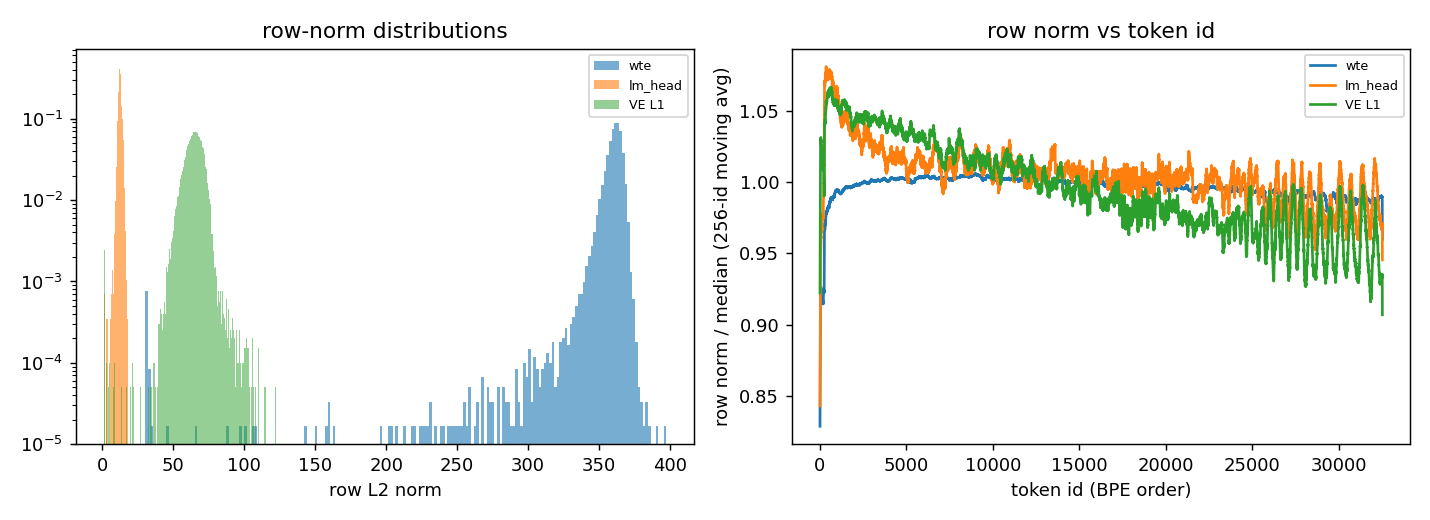
\includegraphics[width=\linewidth]{row_norms.png}
\caption{Left: row-norm distributions of \texttt{wte}, \texttt{lm\_head} and the layer-1 value table (log density). Right: row norm against token id in BPE order, as a 256-id moving average normalised by the median.}
\label{fig:norms}
\end{figure}

\begin{figure}[h]\centering
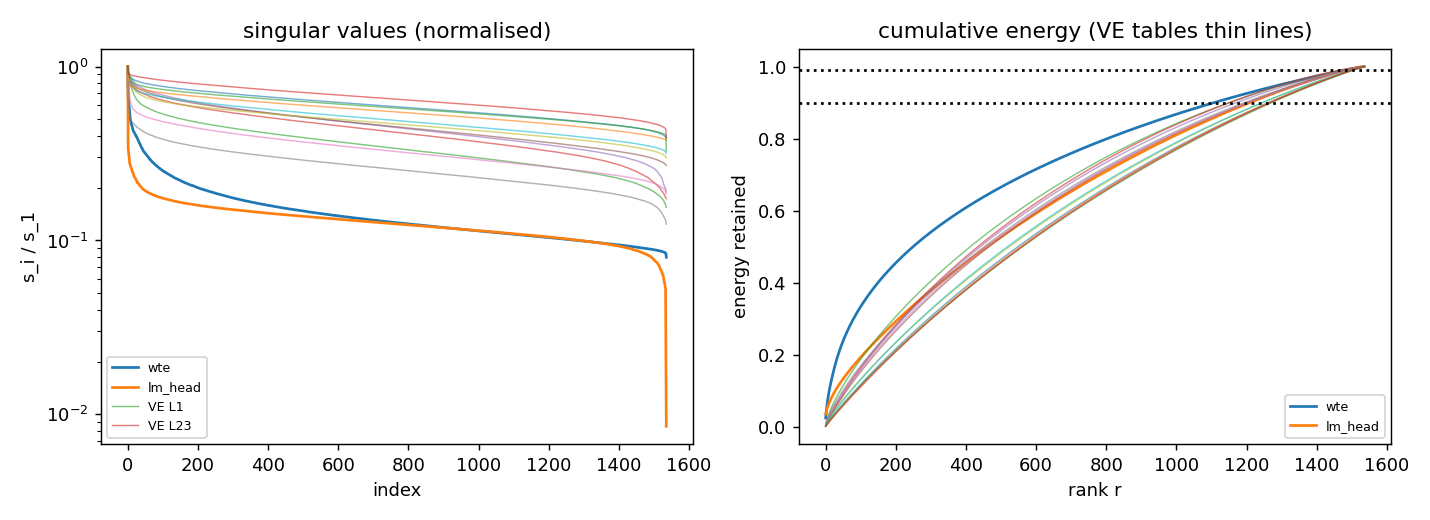
\includegraphics[width=\linewidth]{spectra.png}
\caption{Left: normalised singular values $s_i/s_1$. Right: cumulative energy, with dotted lines at 90\% and 99\%. The value tables (thin lines) are flatter than \texttt{wte}.}
\label{fig:spectra}
\end{figure}

\section{Value embeddings: the headline negative result}
\label{sec:ve}

\subsection{Each table alone}
All 12 tables (layers 1, 3, \ldots, 23) are near-full-rank and isotropic:
\begin{itemize}
\item rank at 99\% energy 1468--1505 of 1536, and at 90\% 1153--1273\meas;
\item participation ratio 1035--1382\meas, rising with depth;
\item mean pairwise cosine $\approx 0.000$\meas\ (centred $-0.0005$);
\item median row norm 64.9--73.6\meas, growing with depth.
\end{itemize}
They are \emph{flatter} than \texttt{wte} (Figure~\ref{fig:spectra}): $s_{\min}/s_{\max}\approx 0.1$--$0.4$, against ${\approx}0.08$ for \texttt{wte}.

\subsection{Cross-table redundancy}
\begin{itemize}
\item Pairwise linear CKA over the 66 pairs: mean \textbf{0.062}\meas\ (p5--p95 0.044--0.092; adjacent value layers 0.068--0.102).
\item After the best orthogonal (Procrustes) alignment, the per-token cosine has median 0.20\meas.
\item \textbf{One shared table + per-layer scalar gate} retains \textbf{9.3\%}\meas. The floor for completely unrelated tables of equal energy is $1/12 = 8.33\%$\der, so the tables share almost nothing.
\item \textbf{One shared table + per-layer $1536{\times}1536$ linear readout} retains \textbf{29.6\%}\meas.
\end{itemize}

\textbf{Definition of ``variance retained''.}
\begin{itemize}
\item Let $X = [V_1 \,|\, \cdots \,|\, V_{12}] \in \mathbb{R}^{32768\times 18432}$ be the concatenation of all 12 tables.
\item With $G = X^\top X$ and eigenvalues $\lambda_1\ge\lambda_2\ge\cdots$ (which are the squared singular values of $X$),
\[
\text{retained}(r) \;=\; \frac{\sum_{i\le r}\lambda_i}{\sum_i \lambda_i} \;=\; 1 - \frac{\|X - X_r\|_F^2}{\|X\|_F^2}
\]
by Eckart--Young, where $X_r$ is the best rank-$r$ approximation.
\item $X_r$ is exactly a shared $r$-dimensional per-token code with per-layer readouts. The measure is computed over the concatenation; it is \emph{not} per-table-then-averaged.
\item It is uncentred (reconstruction energy). The centred variant (column means removed) differs by $\le 0.0003$\meas\ at every rank.
\item The scalar-gate number is the top eigenvalue fraction of the $12\times 12$ Gram matrix of the vectorised tables, i.e.\ the best fit $V_\ell \approx a_\ell T$.
\end{itemize}

\begin{table}[h]\centering\small
\setlength{\tabcolsep}{4pt}
\begin{tabular}{@{}lrrrrrrrr@{}}
\toprule
rank $r$ & 32 & 64 & 128 & 256 & 512 & 1024 & 1536 & 3072 \\
\midrule
Shared code (stacked), retained\meas & 0.016 & 0.027 & 0.0462 & 0.0784 & 0.1324 & 0.2214 & 0.2964 & 0.4742 \\
Per table, no sharing (aggregate)\meas & 0.055 & 0.097 & 0.172 & 0.301 & 0.511 & 0.812 & 1.000 & -- \\
\bottomrule
\end{tabular}
\caption{Variance retained against rank. ``Per table'' truncates each table at rank $r$ separately (own SVD) and aggregates by energy: $\sum_\ell$ retained$_\ell$ / $\sum_\ell$ total$_\ell$. Ranges across tables at $r=512$: 0.464--0.574\meas; at $r=1024$: 0.781--0.851\meas.}
\label{tab:curve}
\end{table}

\begin{figure}[h]\centering
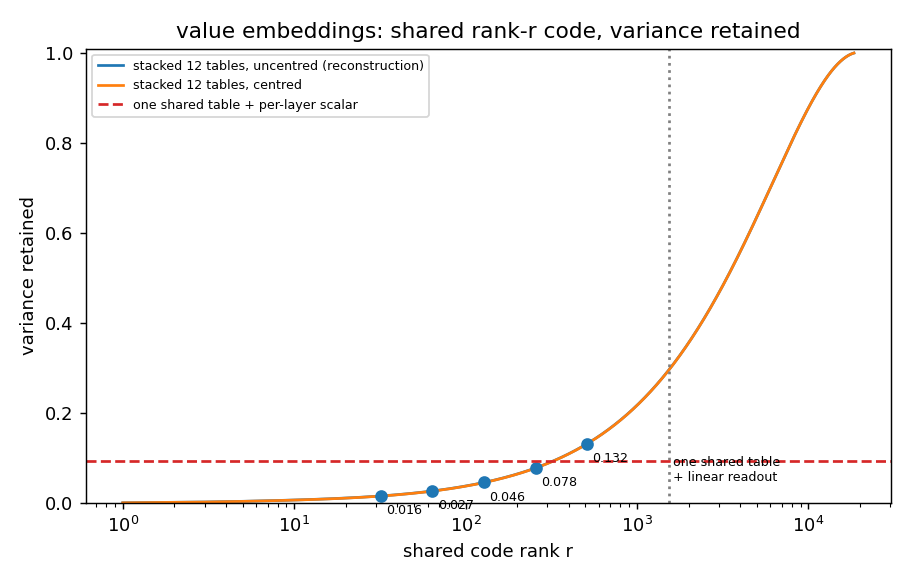
\includegraphics[width=0.85\linewidth]{ve_variance_retained_vs_rank.png}
\caption{Shared rank-$r$ code over the 12 stacked value tables (uncentred and centred, indistinguishable). The dashed line is one shared table + per-layer scalar (0.093). The dotted line at $r=1536$ is one shared table + linear readout (0.296).}
\label{fig:vecurve}
\end{figure}

\subsection{Sharing versus low rank}
Table~\ref{tab:curve} answers the question one way or the other depending on what is held fixed.
\begin{itemize}
\item \textbf{At equal per-layer rank, sharing is expensive.} Per-table $r=512$ retains 51.1\%; a single shared $r=512$ code retains 13.2\%\meas.
\item \textbf{At equal total code size per token, sharing wins.} Per-table $r=256$ uses $12\times256 = 3072$ dimensions per token and retains 30.1\%, against 47.4\% for a shared rank-3072 code\meas. This is guaranteed by Eckart--Young: the block-diagonal per-table approximation is a special case of the stacked rank-$12r$ fit.
\item \textbf{So the binding constraint is low rank itself, not sharing.} Even one table alone needs $r\approx 1024$ to keep 81\%\meas.
\end{itemize}

\subsection{Predictability and quantisation}
\textbf{Not predictable from \texttt{wte}.} The least-squares linear map $\texttt{wte}\to V_\ell$ (centred) explains $R^2 = $ \textbf{0.07--0.09}\meas\ per layer.

\textbf{Product quantisation is poor} (Table~\ref{tab:pq}). k-means with 25 iterations on the trained tables, measured on layers 1, 13 and 23, which agree within $\pm 0.01$.

\begin{table}[h]\centering
\begin{tabular}{@{}lrrrrrr@{}}
\toprule
groups $g\times$ codebook $K$ & $8{\times}256$ & $16{\times}256$ & $48{\times}256$ & $96{\times}256$ & $16{\times}1024$ & $48{\times}1024$ \\
\midrule
relative Frobenius error\meas & 0.97 & 0.94--0.95 & 0.85--0.86 & \textbf{0.74} & 0.92--0.93 & 0.80 \\
\bottomrule
\end{tabular}
\caption{Post-hoc PQ reconstruction error, $\|V - \hat V\|_F/\|V\|_F$. The finest setting tried, 96 sub-spaces of 16 dimensions with 256 codes each, still leaves 74\% error.}
\label{tab:pq}
\end{table}

\subsection{Consequence}
\textbf{Post-hoc low-rank or PQ compression of the value embeddings, which was the original Stage~2a plan of fitting then evaluating, is dead.} The trained tables behave like 12 independent, high-entropy lookups. The open question moves to whether the loss \emph{needs} that content at all. Only the ablation in Section~\ref{sec:stageB}(c) can answer that.

\section{Per-layer structure}
\label{sec:layers}

\begin{figure}[h]\centering
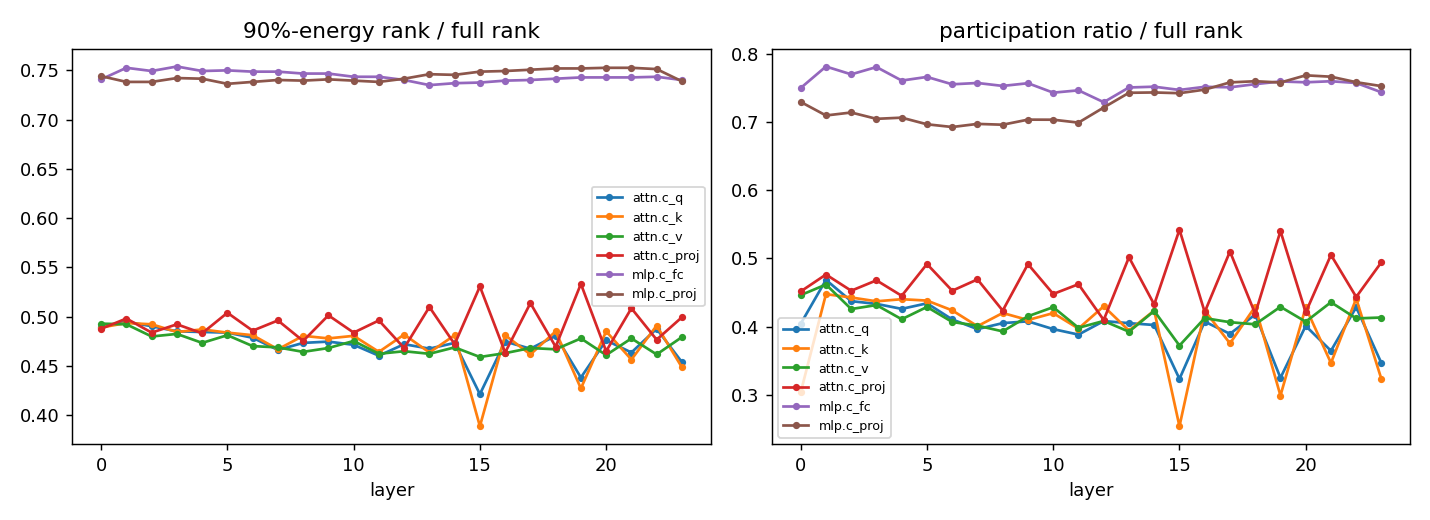
\includegraphics[width=\linewidth]{effective_rank_vs_depth.png}
\caption{Effective rank against depth, as a fraction of full rank. Left: rank at 90\% energy. Right: participation ratio.}
\label{fig:depth}
\end{figure}

\textbf{Effective rank} (Figure~\ref{fig:depth}):
\begin{itemize}
\item The FFN matrices use ${\sim}74$--75\% of their rank at 90\% energy\meas (PR 0.69--0.78).
\item Attention q/k/v/o use ${\sim}39$--53\%\meas (PR 0.25--0.54).
\item \textbf{q/k rank dips sharply at layers 15, 19 and 23} (\texttt{c\_k} PR 0.25 / 0.30 / 0.32 against ${\sim}0.42$ elsewhere\meas). These are full-context 2048-window layers of the SSSL pattern; the dip appears only in the deeper half (layers 3, 7 and 11 do not show it).
\item \textbf{\texttt{attn.c\_proj} rank alternates}: it is higher on exactly the odd layers, which carry value embeddings (PR e.g.\ 0.54 against 0.42\meas).
\end{itemize}

\textbf{No structurally dead ReLU$^2$ units.}
\begin{itemize}
\item In all 24 layers, 0 of 6144 hidden units have an outgoing (\texttt{c\_proj} column) norm below 1\% or 5\% of the layer median\meas.
\item There are 0 exact-zero rows or columns.
\item Outgoing norms are tight: median ${\approx}2.60$, p5 ${\approx}2.30$--2.38\meas.
\item Whether units are dead \emph{on data} is Stage~B(e).
\end{itemize}

\textbf{\texttt{ve\_gate}.}
\begin{itemize}
\item 144 parameters per value-embedding layer, forming $\text{Linear}(12\to 12)$ that maps the first 12 residual channels to one gate per KV head: $g_h = 3\,\sigma(w_h^\top x_{[:12]})\in(0,3)$, with $g_h=1.5$ at $x=0$.
\item Per-head weight norms grow with depth, from 1.8--2.7 at layer 1 to 2.9--9.6 at layer 23\meas. Deep layers therefore make the value-embedding mix-in strongly input-dependent.
\item The actual gate values on data are Stage~B.
\end{itemize}

\textbf{Learned scalars}\meas:
\begin{itemize}
\item \texttt{resid\_lambdas} lie in 0.21--1.10 and rise with depth.
\item \texttt{x0\_lambdas} are large and mixed-sign: 15.7, 9.8 and 5.6 at layers 0--2, and several negative later. The input embedding is re-injected heavily early on.
\item smear $\lambda=0.206$; backout $\lambda=0.179$.
\end{itemize}

\textbf{Sanity}\meas:
\begin{itemize}
\item No NaN or Inf anywhere.
\item Both zero-initialised projections moved well off zero (Frobenius 164--239).
\item \texttt{lm\_head} std went from 0.001 to 0.317, and \texttt{wte} std from 0.8 to 9.19.
\end{itemize}

\section{Incidental finding: 48 never-trained tokens}
48 token ids are still at init scale in \emph{every} value table and in \texttt{wte}\meas:
\begin{itemize}
\item value-table row norm ${\approx}1.0$, the init value;
\item \texttt{wte} row norm ${\approx}30$, against $0.8\sqrt{1536}=31.4$ at init.
\end{itemize}
These are presumably tokens never seen in 5.84\,B training tokens. Dropping them changes the stacked-variance curve and the $R^2$ values by less than $10^{-3}$\meas. Which strings they are has not yet been decoded.

\section{Implications for the LUT programme}
\begin{itemize}
\item \textbf{LUT FFNs} target 32.7\% of parameters\der\ and ${\approx}56.9\%$ of per-token training FLOPs (from the vendored \texttt{estimate\_flops}\der). The FFNs are structurally fully used, so they are the compute target.
\item \textbf{Value embeddings} are 43.6\% of parameters at ${\approx}0\%$ of FLOPs (a gather), and they are \emph{not} cheaply compressible after training. Any saving there is in resident bytes, not compute.
\item The honest cost axis for this component is therefore memory, and any compressed form would have to be trained, not fitted.
\item The existence proof still stands: this architecture already rewards parameter-heavy, compute-light components. The value tables are exactly that.
\end{itemize}

\section{Stage B: data-dependent analysis (to be completed by nebius-h100)}
\label{sec:stageB}
\noindent\fbox{\parbox{0.96\linewidth}{\textbf{This section contains instructions only; replace each subsection body with measured results, keeping the headings.}}}

\medskip\noindent\textbf{Environment.}
\begin{itemize}
\item Stage B needs real forward passes over a held-out shard.
\item This host's tokenizer and validation shard \path{shard_06542} are byte-identical to the run's (sha256-verified against the run manifest). But this GPU (RTX~5090) has no FlashAttention-3, so window-faithful attention maps must run on the H100.
\item The CORE eval bundle is a 26\,MB re-download if needed.
\item \textbf{Run Stage B on nebius-h100 while the instance is still alive.}
\end{itemize}

\subsection*{(a) Attention entropy and effective context length per head}
\textit{Status: not yet run.}

Per head, measure on the val shard:
\begin{itemize}
\item the attention entropy;
\item the effective context length (mean and 90th-percentile attended distance).
\end{itemize}
Split the results by the SSSL window pattern: 18 layers at a 512 window, and 6 at 2048 (the last layer full). Question: do the 2048-window layers actually use their extra range?

\subsection*{(b) Head classification}
\textit{Status: not yet run.}

Classify every head as induction, previous-token, positional, or attention-sink / BOS-dominant. Highest priority:
\begin{itemize}
\item which heads the value embeddings feed (odd layers);
\item whether copy circuits sit where theory says they should.
\end{itemize}

\subsection*{(c) Value-embedding ablation at inference: THE DECISIVE EXPERIMENT}
\textit{Status: not yet run.}

No training is needed.
\begin{itemize}
\item Zero one value table at a time and measure the val bpb change for each of the 12 layers.
\item Also zero all 12 at once.
\item Report each delta against the unablated 0.719\,bpb baseline.
\end{itemize}
This answers whether the 604M value-embedding parameters are needed by the loss at all.

\subsection*{(d) Residual-stream norm growth and logit lens}
\textit{Status: not yet run.}

Measure the residual norm per layer, and apply the logit lens (final norm, then \texttt{lm\_head}) at each layer. Question: at what depth do predictions actually form?

\subsection*{(e) FFN activation statistics under ReLU$^2$}
\textit{Status: not yet run.}

Measure, per layer:
\begin{itemize}
\item the real activation sparsity;
\item how many of the 6144 hidden units fire on any token, and on any token in a batch.
\end{itemize}
Headline number wanted: if the block effectively uses ${\sim}2000$ dimensions, that sizes the LUT replacement.

\end{document}
